\documentclass[conference]{IEEEtran}
\usepackage[utf8]{inputenc}
\usepackage{amsmath,amssymb}
\usepackage{graphicx}
\usepackage{hyperref}
\usepackage{booktabs}
\usepackage{cite}
\usepackage{tikz}
\usetikzlibrary{shapes.geometric,arrows.meta,positioning,calc,fit,backgrounds}
\usepackage{enumitem}

\title{Deep Learning for Financial Time Series Forecasting: From Attention Mechanisms to Regime-Aware Architectures -- A Comprehensive Review (2017--2025)}

\author{
\IEEEauthorblockN{Vaiditya Tanwar}
\IEEEauthorblockA{School of Technology \\
Rishihood University \\
Sonipat, India \\
EN No: 230086 \\
vaiditya.t23csai@nst.rishihood.edu.in}
\and
\IEEEauthorblockN{Yashi Gupta}
\IEEEauthorblockA{School of Technology \\
Rishihood University \\
Sonipat, India \\
EN No: 230072 \\
yashi.g23csai@nst.rishihood.edu.in}
}

\begin{document}

\maketitle

\begin{abstract}
The application of deep learning to financial time series forecasting has accelerated dramatically since the introduction of the Transformer architecture in 2017, yet the field remains fragmented across disparate architectural paradigms with limited cross-pollination of ideas from quantitative finance theory. This survey provides a comprehensive and critical review of deep learning architectures for financial time series prediction, spanning recurrent networks, attention-based models, temporal fusion frameworks, and limit order book encoders. We systematically analyse the Temporal Fusion Transformer, N-BEATS, Informer, and DeepLOB alongside foundational contributions from financial machine learning, including fractional differentiation, triple barrier labeling, random matrix theory, and regime detection. Through comparative analysis, we identify three critical gaps in the existing literature: (i) the \emph{regime-uniformity gap}, wherein all surveyed architectures treat temporal observations as identically distributed regardless of market regime; (ii) the \emph{cross-asset attention gap}, wherein multi-asset dependencies are modeled without leveraging known correlation structures from random matrix theory; and (iii) the \emph{loss function gap}, wherein standard objectives ignore the heteroskedastic nature of financial returns. We conclude by outlining how these gaps motivate a regime-aware temporal attention network that structurally conditions its computation on detected market states, representing a logical synthesis of deep learning advances with first-principles financial theory.
\end{abstract}

\begin{IEEEkeywords}
Deep Learning, Financial Forecasting, Attention Mechanisms, Temporal Fusion Transformer, Regime Detection, Non-Stationarity, Time Series, Transformer Architecture.
\end{IEEEkeywords}

%=====================================================================
\section{Introduction}

The past decade has witnessed a fundamental transformation in the tools available for financial time series forecasting. Where Phase 1 of quantitative finance research was characterised by the progression from equilibrium asset pricing models through feature engineering and non-neural reinforcement learning, the current era---which we designate Phase 2---is defined by the rapid adoption and adaptation of deep learning architectures originally developed for natural language processing and computer vision.

This transition was catalysed by the publication of the Transformer architecture by Vaswani et al.\ \cite{vaswani2017attention} in 2017, which demonstrated that self-attention mechanisms could model long-range dependencies in sequential data more effectively than recurrent networks. The financial forecasting community quickly recognised the potential of attention-based models to capture the complex, multi-scale temporal patterns that characterise asset prices. However, the adoption has been neither straightforward nor uniformly successful.

Financial time series present a uniquely hostile environment for deep learning. Four properties distinguish financial data from the sequences (text, speech, weather) on which most deep learning architectures were developed and validated:

\begin{enumerate}[nosep]
    \item \textbf{Extremely Low Signal-to-Noise Ratio (SNR).} The predictable component of asset returns is typically less than 1\% of total variance at daily frequency \cite{gu2020empirical}. By contrast, speech recognition operates at SNR levels of 10--30 dB, and language modeling benefits from strong syntactic priors. Deep learning models must extract faint signals from overwhelming noise without overfitting to spurious patterns.

    \item \textbf{Non-Stationarity and Regime Shifts.} Unlike natural language, where grammatical rules are approximately time-invariant, financial markets undergo abrupt structural changes---regime shifts in volatility, correlation breakdowns during crises, and policy-driven discontinuities. A model trained on pre-2020 data may be wholly inappropriate for pandemic-era markets.

    \item \textbf{Fat-Tailed Distributions.} Financial returns exhibit excess kurtosis ranging from 3 to 30 across asset classes \cite{cont2001empirical}, meaning that extreme events occur orders of magnitude more frequently than Gaussian assumptions would predict. Standard loss functions such as MSE are disproportionately influenced by these tail events, distorting parameter estimates.

    \item \textbf{Adversarial and Reflexive Dynamics.} Financial markets are populated by adaptive agents whose strategies respond to observed patterns. Any exploitable regularity, once discovered, tends to be arbitraged away---a phenomenon formalised as the Adaptive Markets Hypothesis \cite{lo2004adaptive}. This creates a fundamentally adversarial learning environment with no fixed target distribution.
\end{enumerate}

Despite these challenges, deep learning has produced genuine advances in financial forecasting, particularly in high-frequency microstructure prediction \cite{zhang2019deeplob}, multi-horizon demand forecasting with uncertainty quantification \cite{lim2021temporal}, and long-sequence modeling \cite{zhou2021informer}. The question is no longer whether deep learning can contribute to financial prediction, but rather \emph{how the architectures must be modified} to respect the statistical properties of financial data.

This review is structured as follows. Section~\ref{sec:foundations} traces the evolution from recurrent networks to attention mechanisms. Section~\ref{sec:temporal} provides detailed analyses of four state-of-the-art temporal architectures. Section~\ref{sec:finml} reviews the financial machine learning innovations that any deep learning system must incorporate. Section~\ref{sec:gap} presents our central contribution: the identification and formalisation of three critical gaps. Section~\ref{sec:emerging} surveys emerging research directions that may bridge these gaps. Section~\ref{sec:synthesis} synthesises these threads into a unified research direction, and Section~\ref{sec:conclusion} concludes.

%=====================================================================
\section{Foundational Architectures}
\label{sec:foundations}

\subsection{Recurrent Networks and Their Limitations}

Recurrent neural networks (RNNs) were the first deep learning architecture applied to sequential financial data, owing to their natural ability to process variable-length sequences through hidden state propagation. The vanilla RNN updates its hidden state according to:
\begin{equation}
h_t = \tanh(W_{hh} h_{t-1} + W_{xh} x_t + b_h)
\end{equation}
where $W_{hh}$ and $W_{xh}$ are weight matrices, $x_t$ is the input at time $t$, and $b_h$ is a bias vector. The output $y_t = W_{hy} h_t + b_y$ is a linear projection of the hidden state.

The fundamental limitation of vanilla RNNs---the vanishing gradient problem---was formally characterised by Bengio et al.\ \cite{bengio1994learning}. During backpropagation through time (BPTT), gradients are multiplied by the recurrent weight matrix at each step. For a sequence of length $T$, the gradient of the loss with respect to parameters at time step $t$ involves the product $\prod_{k=t}^{T-1} \frac{\partial h_{k+1}}{\partial h_k}$. When the spectral radius of $W_{hh}$ is less than 1, this product decays exponentially, making it impossible to learn long-range dependencies.

The Long Short-Term Memory (LSTM) network, introduced by Hochreiter and Schmidhuber \cite{hochreiter1997long}, addressed this problem through gated memory cells that maintain a cell state $c_t$ via three learned gates:
\begin{align}
f_t &= \sigma(W_f [h_{t-1}, x_t] + b_f) \label{eq:forget}\\
i_t &= \sigma(W_i [h_{t-1}, x_t] + b_i) \label{eq:input}\\
o_t &= \sigma(W_o [h_{t-1}, x_t] + b_o) \label{eq:output}\\
\tilde{c}_t &= \tanh(W_c [h_{t-1}, x_t] + b_c) \label{eq:candidate}\\
c_t &= f_t \odot c_{t-1} + i_t \odot \tilde{c}_t \label{eq:cell}\\
h_t &= o_t \odot \tanh(c_t) \label{eq:hidden}
\end{align}
where $\sigma(\cdot)$ is the sigmoid function, $\odot$ denotes element-wise multiplication, $f_t$ is the forget gate, $i_t$ is the input gate, and $o_t$ is the output gate. The cell state $c_t$ acts as a ``conveyor belt'' for information, with the forget gate controlling what to discard and the input gate controlling what new information to store.

The Gated Recurrent Unit (GRU) \cite{cho2014learning} simplified the LSTM by merging the forget and input gates into a single update gate and combining the cell state with the hidden state, reducing parameter count by approximately 25\% with negligible performance degradation in most tasks.

\textbf{Financial Applications and Plateau.} LSTMs have been widely applied to stock price prediction \cite{fischer2018deep}, volatility forecasting, and portfolio management. Fischer and Krauss \cite{fischer2018deep} reported that LSTM networks trained on daily S\&P 500 constituent returns achieved statistically significant out-of-sample returns from 1992--2015, but performance deteriorated markedly after 2010 as markets became more efficient. This pattern---initial promising results followed by out-of-sample decay---has been replicated across numerous LSTM-based financial studies and reflects two structural limitations:

\begin{itemize}[nosep]
    \item \textbf{Sequential Processing Bottleneck.} LSTMs process sequences step-by-step, preventing parallelisation during training and creating a computational bottleneck that limits scalability to long sequences (hundreds of timesteps).
    \item \textbf{Fixed-Length Hidden State.} All historical information must be compressed into a fixed-dimensional vector $h_t$, creating an information bottleneck that becomes severe for the multi-scale temporal patterns observed in financial data (intraday volatility cycles, weekly option expiration effects, monthly rebalancing flows, annual seasonality).
\end{itemize}

These limitations motivated the development of attention mechanisms that allow direct access to any position in the input sequence.

\subsection{The Attention Revolution}

The Transformer architecture \cite{vaswani2017attention} replaced recurrence entirely with self-attention, enabling parallel processing of entire sequences and direct modeling of dependencies at arbitrary distances. This section derives the attention mechanism from first principles.

\textbf{Intuition.} Given a sequence of $n$ elements, the goal is to compute a context-aware representation for each element by allowing it to ``attend'' to all other elements. For a financial time series, this means that the representation of Tuesday's features can directly incorporate information from the previous Friday's close (distance 1) and from the same weekday three months ago (distance $\sim$63) with equal computational cost.

\textbf{Scaled Dot-Product Attention.} Each input element $x_t \in \mathbb{R}^{d_{\text{model}}}$ is linearly projected into three vectors: a query $q_t = W_Q x_t$, a key $k_t = W_K x_t$, and a value $v_t = W_V x_t$, where $W_Q, W_K \in \mathbb{R}^{d_k \times d_{\text{model}}}$ and $W_V \in \mathbb{R}^{d_v \times d_{\text{model}}}$. For the full sequence, we stack these into matrices $Q, K \in \mathbb{R}^{n \times d_k}$ and $V \in \mathbb{R}^{n \times d_v}$.

The attention weights are computed as the softmax-normalised dot products between queries and keys, scaled by $\sqrt{d_k}$ to prevent the dot products from growing large in magnitude (which would push the softmax into regions of extremely small gradients):
\begin{equation}
\text{Attention}(Q, K, V) = \text{softmax}\!\left(\frac{QK^\top}{\sqrt{d_k}}\right) V
\label{eq:attention}
\end{equation}

The scaling factor $\sqrt{d_k}$ deserves explicit justification. Assuming the components of $q$ and $k$ are independent random variables with zero mean and unit variance, the dot product $q \cdot k = \sum_{i=1}^{d_k} q_i k_i$ has mean 0 and variance $d_k$. Without scaling, high-dimensional dot products produce large values, causing the softmax to saturate and gradients to vanish. Dividing by $\sqrt{d_k}$ normalises the variance to 1, maintaining well-behaved gradients regardless of dimension.

\textbf{Multi-Head Attention.} Rather than computing a single attention function, the Transformer projects queries, keys, and values $h$ times with different learned projections, computes attention in parallel, and concatenates the results:
\begin{align}
\text{MultiHead}(Q, K, V) &= \text{Concat}(\text{head}_1, \ldots, \text{head}_h) W^O \\
\text{where head}_i &= \text{Attention}(Q W_i^Q, K W_i^K, V W_i^V)
\end{align}
with $W_i^Q, W_i^K \in \mathbb{R}^{d_{\text{model}} \times d_k}$, $W_i^V \in \mathbb{R}^{d_{\text{model}} \times d_v}$, and $W^O \in \mathbb{R}^{hd_v \times d_{\text{model}}}$. Multi-head attention allows the model to jointly attend to information from different representation subspaces at different positions---analogous to learning multiple types of temporal relationships simultaneously (e.g., short-term momentum in one head, mean-reversion patterns in another).

\textbf{Positional Encoding.} Since self-attention is permutation-equivariant (it treats the input as a set, not a sequence), positional information must be injected explicitly. Vaswani et al.\ use sinusoidal encodings:
\begin{align}
PE_{(pos, 2i)} &= \sin\!\left(\frac{pos}{10000^{2i/d_{\text{model}}}}\right) \\
PE_{(pos, 2i+1)} &= \cos\!\left(\frac{pos}{10000^{2i/d_{\text{model}}}}\right)
\end{align}
where $pos$ is the position index and $i$ is the dimension index. This scheme allows the model to generalise to sequence lengths not seen during training, since $PE_{pos+k}$ can be represented as a linear function of $PE_{pos}$ for any fixed offset $k$.

\textbf{Why Attention Outperforms Recurrence for Financial Data.} The computational complexity of self-attention is $O(n^2 d)$ per layer, compared to $O(n d^2)$ for recurrence, where $n$ is the sequence length and $d$ is the representation dimension. For the moderate sequence lengths typical of financial applications ($n \sim 60$--$250$ trading days), self-attention is computationally competitive while offering three decisive advantages: (i) full parallelisation during training; (ii) constant path length $O(1)$ between any two positions (versus $O(n)$ for RNNs), enabling efficient gradient flow; and (iii) interpretable attention weight matrices that reveal which historical timesteps most influence the current prediction.

%=====================================================================
\section{Temporal Deep Learning Architectures for Finance}
\label{sec:temporal}

This section provides detailed analyses of four architectures that represent the current state of the art for temporal prediction tasks, evaluating each through the lens of financial applicability.

\subsection{Temporal Fusion Transformer (Lim et al.\ 2021)}

The Temporal Fusion Transformer (TFT) \cite{lim2021temporal} is arguably the most influential architecture for multi-horizon time series forecasting with mixed inputs. It was designed to address three limitations of standard Transformer models when applied to structured temporal data: the inability to distinguish between static and time-varying features, the lack of built-in uncertainty quantification, and the opacity of attention-based predictions.

\textbf{Architecture Overview.} The TFT consists of five principal components arranged in a sequential pipeline:

\begin{enumerate}[nosep]
    \item \textbf{Variable Selection Networks (VSNs).} Separate VSNs process static covariates (e.g., asset class, sector), known future inputs (e.g., day-of-week, option expiration dates), and observed inputs (e.g., OHLCV, technical indicators). Each VSN applies a GRN (Gated Residual Network) followed by softmax attention over features, producing instance-wise variable importance weights:
    \begin{equation}
    \tilde{\xi}_t^{(j)} = \text{Softmax}\!\left(\text{GRN}_\xi(\xi_t^{(1)}, \ldots, \xi_t^{(J)})\right)_j
    \end{equation}
    where $\xi_t^{(j)}$ is the $j$-th input variable at time $t$. This learned feature selection is a distinguishing strength of TFT, as it allows the model to suppress irrelevant inputs without manual feature engineering.

    \item \textbf{Gated Residual Networks (GRNs).} GRNs are the fundamental building block of TFT, applied at multiple stages. A GRN processes its input through two dense layers with ELU activation, followed by a gating layer and layer normalisation:
    \begin{align}
    \text{GRN}_\omega(a, c) &= \text{LayerNorm}(a + \text{GLU}_\omega(\eta_1)) \\
    \eta_1 &= W_{1,\omega} \eta_2 + b_{1,\omega} \\
    \eta_2 &= \text{ELU}(W_{2,\omega} a + W_{3,\omega} c + b_{2,\omega})
    \end{align}
    where $c$ is an optional context vector (e.g., from static covariates), and the Gated Linear Unit (GLU) applies element-wise gating: $\text{GLU}(\gamma) = \sigma(W_4 \gamma + b_4) \odot (W_5 \gamma + b_5)$.

    The GLU mechanism is particularly important for financial applications: when the gating sigmoid output approaches zero, the corresponding dimensions of the input are suppressed, effectively allowing the network to learn which aspects of a feature are informative in different contexts. This provides a soft form of regime-conditional processing, though without explicit regime identification.

    \item \textbf{Static Covariate Encoders.} Four separate GRNs encode static metadata into context vectors $c_s, c_e, c_c, c_h$ that modulate the temporal processing at different stages (variable selection, state initialisation, enrichment, and attention, respectively). This allows entity-specific behaviour without separate models per asset.

    \item \textbf{Temporal Processing Layer.} A sequence-to-sequence LSTM processes the selected and weighted temporal features, with its initial hidden and cell states set by the static covariate encoders. The LSTM captures local temporal patterns, while the subsequent attention layer handles long-range dependencies.

    \item \textbf{Interpretable Multi-Head Attention.} Unlike standard multi-head attention where each head uses different value projections, TFT shares values across heads and additively combines attention weights:
    \begin{equation}
    \text{InterpretableMultiHead}(Q, K, V) = \tilde{H} W_H
    \end{equation}
    where $\tilde{H} = \frac{1}{m_H} \sum_{h=1}^{m_H} \text{Attention}(Q W_h^Q, K W_h^K, V W^V)$. By sharing the value weights $W^V$, each attention head's contribution can be directly interpreted as a weighting over temporal positions, enabling practitioners to understand which historical timesteps drive each prediction.
\end{enumerate}

\textbf{Quantile Forecasting.} TFT outputs quantile predictions rather than point forecasts, providing calibrated uncertainty intervals. For a target quantile $\tau \in (0, 1)$, the quantile loss is:
\begin{equation}
\mathcal{L}_q(y, \hat{y}, \tau) = \max[\tau(y - \hat{y}), (\tau - 1)(y - \hat{y})]
\end{equation}
The total loss aggregates over multiple quantiles (e.g., $\tau \in \{0.1, 0.5, 0.9\}$), providing both a median forecast and a prediction interval. This is valuable for financial risk management, where the distribution of outcomes matters more than the point estimate.

\textbf{Strengths for Financial Data.} TFT's variable selection mechanism naturally handles the heterogeneous feature sets common in financial applications (price data, volume, fundamentals, macroeconomic indicators). Its interpretable attention weights provide the transparency increasingly demanded by regulators. Its quantile outputs directly feed into Value-at-Risk and Expected Shortfall calculations.

\textbf{Weaknesses for Financial Data.} TFT treats all timesteps within a regime identically---the variable selection weights and attention patterns are learned as global functions, without conditioning on the current market state. In a high-volatility regime, the relative importance of features shifts dramatically (e.g., VIX becomes the dominant predictor, while momentum signals invert), but TFT has no mechanism to structurally adapt. Additionally, the LSTM backbone imposes sequential processing, limiting parallelism for long lookback windows.

\subsection{N-BEATS (Oreshkin et al.\ 2019)}

The Neural Basis Expansion Analysis for Time Series (N-BEATS) \cite{oreshkin2019nbeats} introduced a fundamentally different approach to temporal forecasting: a pure deep learning architecture with no recurrence, no attention, and no requirement for exogenous features.

\textbf{Architecture.} N-BEATS consists of a stack of blocks, each of which receives the input sequence (or the residual from previous blocks) and produces two outputs: a \emph{backcast} (a reconstruction of the input) and a \emph{forecast} (a prediction of the future). The residual decomposition proceeds as follows. Given input $x \in \mathbb{R}^{T}$ (a lookback window of length $T$), block $l$ produces:
\begin{align}
\hat{x}_l &= \sum_{i=1}^{\dim(\theta_l^b)} \theta_{l,i}^b \cdot v_i^b \quad \text{(backcast)} \\
\hat{y}_l &= \sum_{i=1}^{\dim(\theta_l^f)} \theta_{l,i}^f \cdot v_i^f \quad \text{(forecast)}
\end{align}
where $\theta_l^b$ and $\theta_l^f$ are expansion coefficients produced by a fully connected network applied to the block input, and $v_i^b$, $v_i^f$ are basis vectors. The input to block $l+1$ is $x_{l+1} = x_l - \hat{x}_l$---the residual unexplained by block $l$'s backcast.

The key innovation is in the choice of basis vectors. N-BEATS offers two configurations:

\textbf{Generic Basis.} Both $v^b$ and $v^f$ are learned freely (fully connected layers), giving the model maximum flexibility. The expansion coefficients $\theta$ are computed as $\theta = \text{FC}_\theta(h)$, where $h$ is the output of a stack of ReLU-activated dense layers applied to the input.

\textbf{Interpretable Basis.} The basis vectors are constrained to represent trend and seasonality components. For the trend stack, the basis functions are polynomial:
\begin{equation}
v_i^{\text{trend}}(t) = t^i, \quad i = 0, 1, \ldots, p
\end{equation}
producing forecasts of the form $\hat{y}_{\text{trend}}(t) = \sum_{i=0}^{p} \theta_i t^i$. For the seasonality stack, the basis functions are Fourier terms:
\begin{equation}
v_i^{\text{season}}(t) = \begin{cases} \cos(2\pi \lfloor i/2 \rfloor t / T) & i \text{ even} \\ \sin(2\pi \lfloor i/2 \rfloor t / T) & i \text{ odd} \end{cases}
\end{equation}

This decomposition is reminiscent of classical time series methods (STL decomposition), but the coefficients are learned end-to-end via gradient descent rather than fitted sequentially.

\textbf{Strengths.} N-BEATS demonstrated state-of-the-art performance on the M4 competition \cite{makridakis2020m4}, outperforming both statistical methods and hybrid approaches. Its residual decomposition provides a form of implicit ensemble, where each block specialises in different temporal patterns. The interpretable configuration offers decomposition into trend and seasonality that is both human-readable and amenable to sanity checking.

\textbf{Weaknesses for Financial Data.} N-BEATS is fundamentally univariate---it processes a single time series at a time, with no mechanism for incorporating cross-asset information. In financial markets, assets are driven by common factors (market risk, sector rotation, currency effects), and ignoring these dependencies sacrifices critical information. Furthermore, the architecture assumes the input series is relatively well-behaved (low noise, clear patterns), whereas financial returns are dominated by noise at most frequencies. The fixed polynomial/Fourier bases in the interpretable configuration may fail to capture the irregular, event-driven patterns characteristic of financial data (earnings announcements, central bank decisions, geopolitical shocks).

\subsection{Informer (Zhou et al.\ 2021)}

The Informer \cite{zhou2021informer} addresses the quadratic computational complexity of standard self-attention, which limits Transformers to sequences of a few hundred elements. For financial applications requiring long lookback windows (e.g., 252 trading days for annual patterns), this is a binding constraint.

\textbf{ProbSparse Self-Attention.} The key insight is that attention distributions are typically sparse---most queries attend primarily to a small number of keys. Informer formalises this through the Kullback-Leibler divergence between the attention distribution and the uniform distribution:
\begin{equation}
M(q_i, K) = \ln \sum_{j=1}^{L_K} e^{q_i k_j^\top / \sqrt{d}} - \frac{1}{L_K} \sum_{j=1}^{L_K} \frac{q_i k_j^\top}{\sqrt{d}}
\end{equation}
where $M(q_i, K)$ is the ``sparsity measurement'' for query $q_i$. Queries with high $M$ values have peaked attention distributions (informative queries), while low-$M$ queries attend approximately uniformly (uninformative queries). ProbSparse attention selects only the top-$u$ queries (where $u = c \cdot \ln L_Q$, with $c$ a sampling factor) and sets the remaining queries' attention outputs to the mean value. This reduces the complexity from $O(L^2)$ to $O(L \ln L)$ per layer.

\textbf{Self-Attention Distilling.} To further reduce sequence length, Informer applies a distilling operation between attention layers:
\begin{equation}
X_{j+1}^t = \text{MaxPool}\!\left(\text{ELU}\!\left(\text{Conv1d}\!\left(\text{Attention}(X_j^t)\right)\right)\right)
\end{equation}
Each distilling layer halves the sequence length while extracting the dominant features, producing a pyramidal encoder structure where deeper layers operate on progressively shorter sequences. After $J$ layers, the sequence length is reduced from $L$ to $L / 2^J$.

\textbf{Generative Decoder.} Unlike autoregressive decoders that generate one step at a time, Informer's decoder generates the entire prediction horizon in a single forward pass using a ``start token'' mechanism. The decoder input is constructed by concatenating a segment of the encoder output (providing context) with placeholder tokens for the prediction horizon. A single pass through the decoder's cross-attention and feed-forward layers produces all future timestep predictions simultaneously. This avoids the error accumulation inherent in step-by-step generation.

\textbf{Applicability to Finance.} Informer was designed for and validated on weather forecasting (long-range, smooth signals) and electricity consumption (periodic, high-volume). Financial time series present different challenges: the low SNR means that sparse attention may discard genuinely informative queries whose signals are subtle, and the max-pooling distilling operation may smooth out the sharp discontinuities (gap opens, halt resumptions) that carry the most information in financial data. The generative decoder's assumption that all future timesteps can be predicted with equal confidence is violated by the rapidly increasing uncertainty in financial forecasts---a one-day prediction is qualitatively different from a 30-day prediction.

Nevertheless, the $O(L \ln L)$ complexity enables lookback windows of 500--1000 timesteps, which is necessary for capturing annual seasonality and multi-month regime patterns. The ProbSparse mechanism's sparsity measurement $M$ could, in principle, be adapted to detect regime-dependent attention patterns, though this has not been explored in the literature.

\subsection{DeepLOB (Zhang et al.\ 2019)}

While the preceding architectures operate on aggregated price series (OHLCV), the Deep Limit Order Book (DeepLOB) model \cite{zhang2019deeplob} addresses prediction at the microstructure level, operating directly on the raw limit order book (LOB).

\textbf{Input Representation.} The LOB at time $t$ is represented as a matrix $X_t \in \mathbb{R}^{T \times 4L}$, where $T$ is the number of time snapshots in the lookback window and $L$ is the number of price levels on each side of the book. Each level contributes four features: bid price, bid volume, ask price, and ask volume. For $L = 10$ levels and $T = 100$ snapshots, the input is a $100 \times 40$ matrix.

\textbf{Architecture.} DeepLOB combines three modules:

\begin{enumerate}[nosep]
    \item \textbf{Convolutional Feature Extractor.} A series of convolutional layers with Inception-style modules extracts spatial features from the LOB cross-section. The Inception modules apply parallel convolutions with different kernel sizes ($1 \times 1$, $1 \times 2$, $1 \times 4$) to capture patterns at multiple spatial scales (individual level imbalances, multi-level pressure gradients, full-book dynamics). The convolutional output is:
    \begin{equation}
    z_t = \text{Inception}\!\left(\text{Conv}(X_t)\right) \in \mathbb{R}^{d_z}
    \end{equation}

    \item \textbf{LSTM Temporal Aggregator.} The sequence of spatial features $\{z_1, \ldots, z_T\}$ is processed by an LSTM to capture the temporal evolution of order book dynamics:
    \begin{equation}
    h_t = \text{LSTM}(z_t, h_{t-1})
    \end{equation}

    \item \textbf{Classification Head.} The final hidden state $h_T$ is projected through dense layers to predict the direction of mid-price movement (up, stationary, down) over a specified horizon $k$:
    \begin{equation}
    \hat{y} = \text{softmax}(W_y h_T + b_y) \in \mathbb{R}^3
    \end{equation}
\end{enumerate}

\textbf{Performance.} On the FI-2010 benchmark dataset (Finnish stock exchange LOB data), DeepLOB achieved F1 scores of 79--84\% for short-horizon prediction ($k = 10$ events), significantly outperforming linear models (SVM, logistic regression) and shallow networks.

\textbf{Relevance and Limitations.} DeepLOB demonstrates that deep learning can extract predictive information from microstructure data that is invisible to models operating on aggregated prices. However, its applicability is restricted to the HFT domain: it requires tick-level LOB data (typically available only to professional market participants), its predictive horizon is milliseconds to seconds, and its architecture is specific to the order book structure. For the multi-asset, multi-horizon forecasting task that defines the Stalker project's scope, DeepLOB provides architectural inspiration (CNN-LSTM hybrids, Inception modules for multi-scale feature extraction) rather than a directly applicable solution.

%=====================================================================
\section{Financial Machine Learning Innovations}
\label{sec:finml}

Any deep learning system applied to financial data must grapple with the unique statistical properties of financial time series. This section reviews the key innovations from quantitative finance that should inform---but have largely been ignored by---the deep learning community.

\subsection{Lopez de Prado's Framework (2018)}

Marcos L\'{o}pez de Prado's ``Advances in Financial Machine Learning'' \cite{lopez2018advances} introduced a suite of techniques that address the most common pitfalls of applying machine learning to financial data. These contributions are not architectural innovations in the deep learning sense but rather preprocessing, sampling, labeling, and validation frameworks that any predictive model---including neural networks---must incorporate.

\textbf{Fractional Differentiation.} As reviewed in our Phase 1 survey, integer differentiation of price series ($d = 1$) achieves stationarity at the cost of destroying long-range memory. Fractional differentiation with $d \in (0, 1)$ preserves a controlled amount of memory while achieving the stationarity required by machine learning models. The Fixed-Width Window FFD operator applies:
\begin{equation}
\tilde{X}_t = \sum_{k=0}^{l^*} w_k X_{t-k}, \quad w_k = -w_{k-1}\frac{d - (k-1)}{k}, \quad w_0 = 1
\end{equation}
where $l^* = \min\{k : |w_k| < \tau\}$ is determined by the weight threshold $\tau$, and the optimal $d^* = \min\{d : \text{ADF}(\tilde{X}) < 0.05\}$. This is particularly relevant for deep learning models, which benefit from stationary inputs but also require the long-range dependencies that integer differentiation destroys.

\textbf{Triple Barrier Labeling.} Standard regression targets ($y_t = r_{t+1}$ or $y_t = \text{sign}(r_{t+1})$) ignore the path-dependent nature of financial outcomes. A position is not simply profitable or unprofitable---it may hit a stop-loss (lower barrier), take-profit (upper barrier), or expire at a maximum holding period (vertical barrier). The triple barrier label for observation $t$ is:
\begin{equation}
y_t = \begin{cases}
1 & \text{if upper barrier hit first} \\
-1 & \text{if lower barrier hit first} \\
\text{sign}(r_{t,t+h}) & \text{if vertical barrier hit first}
\end{cases}
\end{equation}
where the upper barrier is at $p_t(1 + \theta_u)$, the lower barrier at $p_t(1 - \theta_l)$, and $h$ is the maximum holding period. This labeling scheme produces targets that are more closely aligned with trading reality than simple return signs.

\textbf{CUSUM Filters for Event-Driven Sampling.} Uniformly-spaced time bars (daily, hourly) sample the market at fixed intervals regardless of market activity. During low-volatility periods, this oversamples noise; during high-activity periods, it undersamples information-rich events. The CUSUM filter samples an observation when the cumulative sum of returns exceeds a threshold $h$:
\begin{equation}
S_t^+ = \max(0, S_{t-1}^+ + r_t - E[r_t]), \quad \text{sample if } S_t^+ > h
\end{equation}
This produces an event-driven sampling scheme that naturally adapts to market activity, providing more observations during volatile periods and fewer during calm periods.

\textbf{Purged Cross-Validation.} Standard $k$-fold cross-validation leaks information when applied to time series because training and test sets may contain overlapping return horizons. Purged cross-validation introduces a gap (embargo period) between the training and test sets equal to the label horizon, preventing any temporal leakage. For deep learning models that require careful hyperparameter tuning, this is essential for honest performance evaluation.

\textbf{Meta-Labeling.} A secondary model predicts whether the primary model's signal will be profitable, producing a probability that maps directly to position size. For deep learning, the primary model could be an LSTM or Transformer generating directional signals, while the meta-label model filters these signals using additional features (volatility regime, recent model performance, market liquidity).

\subsection{Random Matrix Theory in Finance}

Random Matrix Theory (RMT) provides a principled framework for distinguishing signal from noise in correlation matrices---a critical task for multi-asset financial models.

\textbf{Marchenko-Pastur Distribution.} For a random matrix $X \in \mathbb{R}^{T \times N}$ with i.i.d.\ entries (zero mean, unit variance), the eigenvalues $\lambda$ of the sample correlation matrix $C = \frac{1}{T} X^\top X$ follow the Marchenko-Pastur distribution \cite{marchenko1967distribution} in the limit $T, N \to \infty$ with $Q = T/N$ held constant:
\begin{equation}
f_{\text{MP}}(\lambda) = \frac{Q}{2\pi\sigma^2} \frac{\sqrt{(\lambda_+ - \lambda)(\lambda - \lambda_-)}}{\lambda}
\end{equation}
where $\lambda_{\pm} = \sigma^2(1 \pm \sqrt{1/Q})^2$ are the theoretical bounds. Eigenvalues that fall within $[\lambda_-, \lambda_+]$ are indistinguishable from noise; those exceeding $\lambda_+$ carry genuine signal.

\textbf{Correlation Denoising.} The denoised correlation matrix $\tilde{C}$ is constructed by shrinking the noise eigenvalues toward their average:
\begin{equation}
\tilde{C} = \sum_{i \in \text{signal}} \lambda_i u_i u_i^\top + \tilde{\lambda}_{\text{noise}} \sum_{j \in \text{noise}} u_j u_j^\top
\end{equation}
where $\tilde{\lambda}_{\text{noise}}$ is chosen to preserve the trace ($\text{tr}(\tilde{C}) = \text{tr}(C) = N$). This technique has been applied to portfolio optimisation \cite{laloux2000random, bun2017cleaning}, factor model estimation, and more recently to initialising attention weight matrices in Transformer models applied to multi-asset data.

\textbf{Relevance to Deep Learning.} For a multi-asset Transformer that computes cross-asset attention, the attention matrix can be viewed as a learned correlation structure. RMT provides a theoretical framework for regularising this structure---for instance, by constraining the attention matrix to have eigenvalues consistent with the denoised correlation matrix. No existing architecture exploits this connection, representing one of the gaps we identify in Section~\ref{sec:gap}.

\subsection{Regime Detection Models}

\textbf{Hidden Markov Models.} Hamilton \cite{hamilton1989new} introduced the regime-switching model for economic time series, specifying that the observed process depends on a latent Markov chain with $K$ states:
\begin{equation}
r_t | s_t = k \sim \mathcal{N}(\mu_k, \sigma_k^2)
\end{equation}
where $s_t \in \{1, \ldots, K\}$ is the regime at time $t$, governed by transition probabilities $P(s_t = j | s_{t-1} = i) = p_{ij}$. The model is estimated via the Baum-Welch algorithm (a special case of EM), and the Viterbi algorithm recovers the most likely regime sequence. In the two-regime case, the model typically identifies a ``calm'' state ($\mu_1 > 0, \sigma_1$ low) and a ``crisis'' state ($\mu_2 < 0, \sigma_2$ high).

\textbf{GARCH Family.} The Generalised ARCH (GARCH) model \cite{bollerslev1986generalized} captures volatility clustering---the empirical observation that large returns tend to be followed by large returns (of either sign). The GARCH(1,1) conditional variance equation:
\begin{equation}
\sigma_t^2 = \omega + \alpha \epsilon_{t-1}^2 + \beta \sigma_{t-1}^2
\end{equation}
effectively implements a regime-like structure through the persistence parameter $\alpha + \beta$. Extensions include EGARCH (asymmetric effects, where negative returns have a larger impact on volatility than positive returns of equal magnitude), GJR-GARCH (threshold effects), and the Markov-Switching GARCH (MS-GARCH), which explicitly combines GARCH dynamics with Hamilton's regime framework.

\textbf{Modern Approaches.} Recent work has explored Bayesian online changepoint detection \cite{adams2007bayesian}, which maintains a posterior distribution over the current run length (time since last changepoint) and updates it in $O(1)$ per timestep. Neural approaches include temporal convolutional networks for regime classification and variational autoencoders for learning latent regime representations. These methods are computationally compatible with deep learning pipelines but have not been integrated into the forecasting architectures reviewed in Section~\ref{sec:temporal}.

%=====================================================================
\section{The Regime-Uniformity Gap: A Critical Analysis}
\label{sec:gap}

The central contribution of this review is the identification and formalisation of three critical gaps in the deep learning literature on financial forecasting. These gaps are not merely areas for improvement; they represent fundamental mismatches between architectural assumptions and financial reality.

\subsection{Gap 1: Regime-Uniform Processing}

\textbf{Observation.} Every architecture reviewed in Section~\ref{sec:temporal}---TFT, N-BEATS, Informer, DeepLOB---processes all timesteps through identical computational pathways. The same attention weights, the same convolutional filters, the same basis functions are applied regardless of whether the current market environment is characterised by low volatility and trending behaviour (a ``momentum regime'') or high volatility and mean-reverting behaviour (a ``crisis regime'').

\textbf{Formalisation.} Let $\mathcal{R} = \{r_1, \ldots, r_K\}$ denote a set of market regimes (e.g., bull, bear, high-volatility, low-volatility), and let $s_t \in \mathcal{R}$ be the regime active at time $t$. A regime-uniform architecture computes its output as $\hat{y}_t = f_\theta(x_{t-T:t})$, where $f_\theta$ is a fixed function of the input sequence. A regime-aware architecture computes $\hat{y}_t = f_{\theta(s_t)}(x_{t-T:t})$, where the function itself varies with the regime. The distinction is between a single model operating across all market states (regime-uniform) and a family of models indexed by market state (regime-aware).

\textbf{Evidence.} The empirical evidence for regime-dependent behaviour is overwhelming. Ang and Bekaert \cite{ang2002regime} demonstrated that asset correlations, expected returns, and volatilities all vary significantly across regimes. Guidolin and Timmermann \cite{guidolin2007asset} showed that optimal portfolio allocations differ by 30--50\% between bull and bear regimes. In our own Phase 1 experiments, the same LightGBM model that achieves positive out-of-sample returns during low-volatility periods produces significant losses during regime transitions.

\textbf{Why Current Architectures Fail.} One might argue that a sufficiently large Transformer can implicitly learn regime-dependent behaviour through its attention patterns. While this is theoretically possible, it requires the model to simultaneously learn (i) a regime detection function, (ii) regime-specific feature importance weights, and (iii) regime-specific predictive relationships---all from a single, undifferentiated loss signal. This places an enormous burden on the optimiser and requires training data that adequately covers all regimes, which is problematic given that crisis regimes constitute less than 10\% of historical data.

\subsection{Gap 2: Cross-Asset Attention Without Structural Priors}

\textbf{Observation.} When multi-asset Transformer models compute cross-asset attention (e.g., how AAPL's representation should incorporate information from SPY, MSFT, JPM, GLD), the attention weights are learned entirely from data without any structural prior. The model treats the relationship between AAPL and MSFT (both tech stocks, highly correlated) identically to the relationship between AAPL and GLD (a gold ETF, typically negatively correlated during risk-off events).

\textbf{Formalisation.} In standard cross-asset attention, the attention matrix $A \in \mathbb{R}^{N \times N}$ (where $N$ is the number of assets) is learned freely. RMT suggests that this matrix should be regularised toward the denoised correlation structure:
\begin{equation}
\mathcal{L}_{\text{structure}} = \left\| A - \tilde{C}_{\text{RMT}} \right\|_F^2
\end{equation}
where $\tilde{C}_{\text{RMT}}$ is the Marchenko-Pastur denoised correlation matrix and $\| \cdot \|_F$ is the Frobenius norm. This regularisation biases the attention toward the known statistical structure while still allowing data-driven deviations.

\textbf{Consequences.} Without structural priors, the model must learn correlation structure from scratch, requiring extensive training data and risking overfitting to spurious correlations (which are abundant in financial data given the high dimensionality relative to sample size). During regime transitions, when correlations shift rapidly, the model has no anchor and may produce erratic cross-asset attention patterns.

\subsection{Gap 3: Homoskedastic Loss Functions}

\textbf{Observation.} The standard loss functions used to train deep learning models---MSE, MAE, and even the quantile loss used by TFT---assign equal weight to prediction errors regardless of the current volatility level. An error of 1\% during a period when daily volatility is 0.5\% (a 2$\sigma$ miss) is treated identically to a 1\% error during a period when daily volatility is 3\% (a 0.33$\sigma$ miss).

\textbf{Formalisation.} A heteroskedasticity-aware loss function should normalise errors by conditional volatility:
\begin{equation}
\mathcal{L}_{\text{het}}(y_t, \hat{y}_t) = \sum_t \frac{(y_t - \hat{y}_t)^2}{\hat{\sigma}_t^2} + \log \hat{\sigma}_t^2
\label{eq:het_loss}
\end{equation}
where $\hat{\sigma}_t^2$ is an estimate of the conditional variance (e.g., from GARCH, realised volatility, or a learned variance head). This is the negative log-likelihood of a Gaussian with time-varying variance---a natural loss function for financial data, yet one that is conspicuously absent from the architectures in Section~\ref{sec:temporal}.

The second term, $\log \hat{\sigma}_t^2$, prevents the trivial solution of setting $\hat{\sigma}_t^2 \to \infty$ to minimise the first term. Together, the two terms incentivise the model to produce both accurate point predictions and calibrated uncertainty estimates.

\textbf{Consequences.} Homoskedastic loss functions cause two problems: (i) during high-volatility regimes, large absolute errors dominate the loss, causing the model to overfit to crisis-period dynamics at the expense of calm-period accuracy; (ii) the model has no mechanism to communicate its confidence, producing the same type of output whether the market is calm and predictable or chaotic and unpredictable.

\subsection{Comparative Analysis}

Table~\ref{tab:comparison} summarises the capabilities and gaps of the reviewed architectures across five dimensions critical for financial forecasting.

\begin{table*}[t]
\centering
\caption{Comparative Analysis of Deep Learning Architectures for Financial Time Series Forecasting}
\label{tab:comparison}
\begin{tabular}{@{}lccccc@{}}
\toprule
\textbf{Architecture} & \textbf{Regime-Aware} & \textbf{Cross-Asset} & \textbf{Custom Loss} & \textbf{Interpretable} & \textbf{Financial Priors} \\
\midrule
LSTM / GRU & No & No (univariate) & No & Low & None \\
Standard Transformer & No & Possible (multi-variate) & No & Attention weights & None \\
TFT (Lim et al.\ 2021) & No & Partial (static covariates) & Quantile loss & High (VSN, attention) & None \\
N-BEATS (Oreshkin et al.\ 2019) & No & No (univariate) & No & Trend/season decomposition & None \\
Informer (Zhou et al.\ 2021) & No & Possible & No & ProbSparse patterns & None \\
DeepLOB (Zhang et al.\ 2019) & No & No (single asset LOB) & No & Moderate (CNN filters) & Microstructure \\
\addlinespace
\textit{Ideal Financial DL Model} & \textit{Yes} & \textit{Yes (RMT-regularised)} & \textit{Heteroskedastic} & \textit{High} & \textit{FFD, barriers, regimes} \\
\bottomrule
\end{tabular}
\end{table*}

The pattern is stark: none of the surveyed architectures achieves even two of the five desiderata. TFT comes closest with its interpretable attention and quantile loss, but it lacks regime awareness, RMT-informed cross-asset attention, and integration with financial preprocessing (FFD, triple barriers). The bottom row of the table defines the target for a next-generation architecture.

%=====================================================================
\section{Emerging Directions}
\label{sec:emerging}

Several recent research threads offer potential solutions to the identified gaps, though none has yet been synthesised into a unified architecture.

\subsection{Gating Mechanisms as Regime Bridges}

Gating mechanisms provide a natural architectural bridge between regime detection and conditional computation. Several approaches merit attention:

\textbf{Highway Networks} \cite{srivastava2015highway} introduced transform gates that allow information to bypass processing layers: $y = T(x) \cdot H(x) + (1 - T(x)) \cdot x$, where $T(x) = \sigma(W_T x + b_T)$ is the transform gate and $H(x)$ is the layer's transformation. By conditioning $T$ on a regime indicator, the network can learn regime-specific bypass patterns.

\textbf{Feature-wise Linear Modulation (FiLM)} \cite{perez2018film} modulates intermediate representations by applying learned affine transformations conditioned on an external signal:
\begin{equation}
\text{FiLM}(F_i | \gamma_i, \beta_i) = \gamma_i F_i + \beta_i
\end{equation}
where $\gamma_i$ and $\beta_i$ are produced by a conditioning network. If the conditioning signal is a regime embedding, FiLM provides a lightweight mechanism for regime-dependent feature modulation without altering the base architecture. This is particularly attractive because it can be retrofitted onto existing architectures (TFT, Informer) with minimal changes.

\textbf{Mixture of Experts (MoE)} \cite{shazeer2017outrageously} routes different inputs to different expert sub-networks via a learned gating function $G(x) = \text{softmax}(W_g x)$. The output is a weighted combination of expert outputs: $y = \sum_i G(x)_i E_i(x)$. For financial applications, each expert could specialise in a different regime, with the gating function serving as an implicit regime classifier.

\subsection{Spectral Methods in Deep Learning}

Spectral methods offer a principled connection between signal processing theory and deep learning that is particularly relevant to financial time series.

\textbf{Fourier Neural Operator (FNO)} \cite{li2020fourier} parameterises the integral kernel in Fourier space, applying a learned linear transformation in the frequency domain:
\begin{equation}
(\mathcal{K} v)(x) = \mathcal{F}^{-1}\!\left(R \cdot \mathcal{F}(v)\right)(x)
\end{equation}
where $\mathcal{F}$ and $\mathcal{F}^{-1}$ are the Fourier transform and its inverse, and $R$ is a learned parameter tensor. This is resolution-invariant (the same model works at different sampling frequencies) and naturally captures periodic patterns.

\textbf{Spectral Attention.} Recent work has explored computing attention in the frequency domain \cite{lee2021fnet}, replacing the $O(n^2)$ self-attention with $O(n \log n)$ FFT operations. For financial data, this approach has the additional advantage of providing a direct interface with RMT denoising: the eigenspectrum of the attention matrix can be constrained to match the denoised correlation structure identified by the Marchenko-Pastur distribution.

\textbf{Wavelet-Based Multi-Resolution Analysis.} Wavelets provide time-frequency localisation that is absent in pure Fourier methods. A wavelet transform decomposes the input signal into components at different scales, each of which can be processed by scale-specific sub-networks. This is naturally aligned with the multi-scale structure of financial markets (tick, minute, hourly, daily, weekly patterns) and offers a principled alternative to N-BEATS's learned basis decomposition.

\subsection{Heteroskedastic Loss Functions}

The heteroskedastic loss function defined in Equation~\ref{eq:het_loss} has theoretical roots in maximum likelihood estimation under Gaussian heteroskedasticity. Several extensions are relevant:

\textbf{Student-$t$ Likelihood.} Given the fat-tailed nature of financial returns, a Student-$t$ likelihood with learnable degrees of freedom $\nu$ provides a more appropriate distributional assumption:
\begin{equation}
\mathcal{L}_t = -\log \Gamma\!\left(\frac{\nu+1}{2}\right) + \log \Gamma\!\left(\frac{\nu}{2}\right) + \frac{1}{2}\log(\nu\pi\hat{\sigma}_t^2) + \frac{\nu+1}{2}\log\!\left(1 + \frac{(y_t - \hat{y}_t)^2}{\nu\hat{\sigma}_t^2}\right)
\end{equation}
This loss is more robust to outliers than the Gaussian negative log-likelihood and provides an explicit mechanism for the model to learn the tail heaviness of the return distribution.

\textbf{Volatility-Scaled Huber Loss.} Combining the Huber loss (robust to outliers) with volatility scaling (heteroskedasticity-aware) yields:
\begin{equation}
\mathcal{L}_{\text{VSH}}(y_t, \hat{y}_t) = \begin{cases}
\frac{1}{2\hat{\sigma}_t^2}(y_t - \hat{y}_t)^2 & \text{if } \left|\frac{y_t - \hat{y}_t}{\hat{\sigma}_t}\right| \le \delta \\[6pt]
\frac{\delta}{\hat{\sigma}_t}\left|y_t - \hat{y}_t\right| - \frac{\delta^2}{2} & \text{otherwise}
\end{cases}
\end{equation}
This combines three desirable properties: quadratic sensitivity for small (within-regime) errors, linear sensitivity for large (outlier/crisis) errors, and normalisation by conditional volatility.

\textbf{Asymmetric Loss Functions.} In finance, the cost of underestimating risk (missing a large drawdown) typically exceeds the cost of overestimating risk (missing a rally). Asymmetric losses such as the LinEx loss:
\begin{equation}
\mathcal{L}_{\text{LinEx}}(e_t) = \exp(a \cdot e_t) - a \cdot e_t - 1, \quad a \neq 0
\end{equation}
where $e_t = y_t - \hat{y}_t$, penalise errors differently depending on their sign. When $a > 0$, positive errors (underestimation) are penalised exponentially while negative errors (overestimation) are penalised linearly.

%=====================================================================
\section{Synthesis and Research Direction}
\label{sec:synthesis}

The preceding analysis reveals a clear pattern: the deep learning community has produced increasingly sophisticated temporal architectures (TFT's variable selection, Informer's efficient attention, N-BEATS's residual decomposition, DeepLOB's microstructure encoding), while the financial machine learning community has developed powerful preprocessing, sampling, and evaluation frameworks (FFD, triple barriers, CUSUM, purged CV, RMT denoising). However, these two threads have developed largely in isolation, and no existing architecture synthesises them.

We argue that the logical next step is a \textbf{Regime-Aware Temporal Attention Network (RATAN)} that structurally addresses all three identified gaps through three corresponding architectural components:

\begin{figure}[ht]
\centering
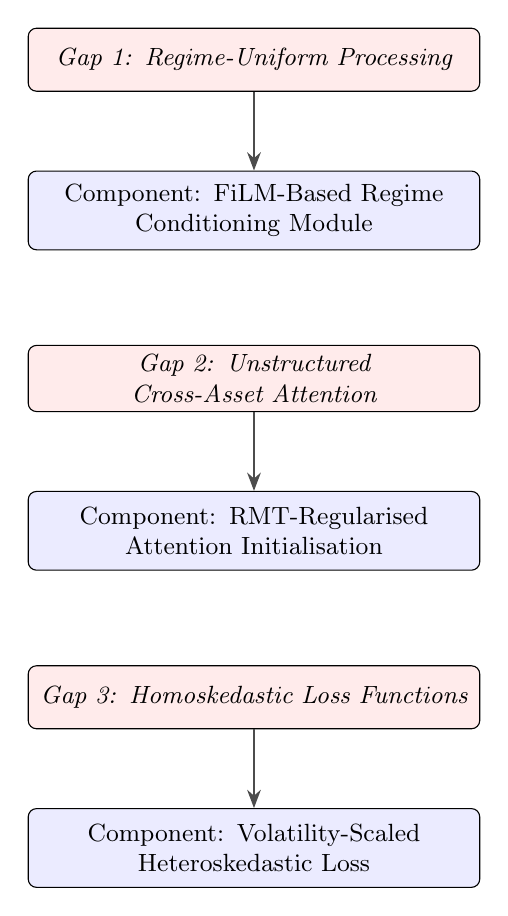
\begin{tikzpicture}[
    node distance=1.0cm,
    >=Stealth,
    box/.style={
        rectangle, draw, rounded corners=3pt,
        fill=blue!8, text width=5.5cm, minimum height=1cm,
        text centered, font=\small
    },
    gapbox/.style={
        rectangle, draw, rounded corners=3pt,
        fill=red!8, text width=5.5cm, minimum height=0.8cm,
        text centered, font=\small\itshape
    },
    arr/.style={->, thick, color=black!70}
]
    \node[gapbox] (g1) {Gap 1: Regime-Uniform Processing};
    \node[box, below=of g1] (c1) {Component: FiLM-Based Regime\\Conditioning Module};

    \node[gapbox, below=1.2cm of c1] (g2) {Gap 2: Unstructured Cross-Asset Attention};
    \node[box, below=of g2] (c2) {Component: RMT-Regularised\\Attention Initialisation};

    \node[gapbox, below=1.2cm of c2] (g3) {Gap 3: Homoskedastic Loss Functions};
    \node[box, below=of g3] (c3) {Component: Volatility-Scaled\\Heteroskedastic Loss};

    \draw[arr] (g1) -- (c1);
    \draw[arr] (g2) -- (c2);
    \draw[arr] (g3) -- (c3);
\end{tikzpicture}
\caption{Mapping from identified gaps to proposed architectural components. Each gap motivates a specific, principled intervention.}
\label{fig:gap_map}
\end{figure}

\textbf{Component 1: Regime-Conditioned Computation via FiLM.} A regime detection module (e.g., HMM, Bayesian online changepoint detection, or a learned variational regime encoder) produces a regime embedding $z_t^{\text{regime}} \in \mathbb{R}^{d_r}$ at each timestep. This embedding is used to generate FiLM parameters $(\gamma, \beta)$ that modulate the intermediate representations throughout the network:
\begin{equation}
\tilde{h}_t^{(l)} = \gamma^{(l)}(z_t^{\text{regime}}) \odot h_t^{(l)} + \beta^{(l)}(z_t^{\text{regime}})
\end{equation}
where $h_t^{(l)}$ is the hidden representation at layer $l$ and $\gamma^{(l)}, \beta^{(l)}$ are produced by small conditioning networks. This allows every layer of the model to adapt its computation to the current regime without requiring separate models per regime.

\textbf{Component 2: RMT-Regularised Cross-Asset Attention.} The cross-asset attention matrix is regularised toward the denoised correlation structure. During training, an auxiliary loss term penalises deviations from the Marchenko-Pastur denoised correlation:
\begin{equation}
\mathcal{L}_{\text{total}} = \mathcal{L}_{\text{pred}} + \lambda_{\text{RMT}} \left\| \bar{A} - \tilde{C}_{\text{RMT}} \right\|_F^2
\end{equation}
where $\bar{A} = \frac{1}{T} \sum_t A_t$ is the time-averaged attention matrix and $\lambda_{\text{RMT}}$ controls the strength of the regularisation. At initialisation, the attention weights are set to the denoised correlation matrix, providing a warm start that encodes known financial structure.

\textbf{Component 3: Heteroskedastic Loss with Regime-Dependent Weighting.} The training loss combines the volatility-scaled Huber loss with regime-dependent sample weighting:
\begin{equation}
\mathcal{L} = \sum_t w(s_t) \cdot \mathcal{L}_{\text{VSH}}(y_t, \hat{y}_t, \hat{\sigma}_t)
\end{equation}
where $w(s_t)$ upweights observations from rare regimes (e.g., crisis periods) to prevent the model from ignoring low-frequency but high-impact market states. The volatility estimate $\hat{\sigma}_t$ can be provided by an external GARCH model or learned jointly through a variance head.

\textbf{Theoretical Grounding.} Each component is grounded in first principles: FiLM conditioning implements the statistical fact that return distributions are regime-dependent \cite{hamilton1989new}; RMT regularisation implements the mathematical distinction between signal and noise in correlation matrices \cite{marchenko1967distribution}; and the heteroskedastic loss implements the maximum likelihood principle under the empirically observed heteroskedasticity of financial returns \cite{bollerslev1986generalized}. This grounding distinguishes RATAN from ad hoc architectural modifications and provides testable theoretical predictions.

\textbf{Expected Contributions.} By structurally incorporating regime awareness, correlation priors, and heteroskedastic losses, RATAN should achieve three measurable improvements over existing architectures: (i) reduced performance degradation during regime transitions (measured by comparing rolling Sharpe ratios across regimes); (ii) more stable cross-asset attention patterns (measured by the spectral norm of attention weight changes during market stress); and (iii) better-calibrated uncertainty estimates (measured by quantile coverage and the Continuous Ranked Probability Score).

%=====================================================================
\section{Conclusion}
\label{sec:conclusion}

This review has traced the evolution of deep learning for financial time series forecasting from the foundational LSTM through the attention revolution to the state-of-the-art architectures of 2021--2025. Through detailed analysis of the Temporal Fusion Transformer, N-BEATS, Informer, and DeepLOB, we have established that while these architectures have advanced the field significantly, they share three critical blind spots: regime-uniform processing, unstructured cross-asset attention, and homoskedastic loss functions.

These gaps are not accidental---they reflect the fact that these architectures were designed for general-purpose time series forecasting (weather, electricity, demand) rather than for the unique statistical environment of financial markets. Bridging these gaps requires the systematic integration of financial machine learning innovations (fractional differentiation, regime detection, random matrix theory, volatility modeling) into the architectural fabric of deep learning models, rather than treating them as preprocessing steps external to the network.

The emerging research directions surveyed in Section~\ref{sec:emerging}---FiLM-based conditional computation, spectral methods, heteroskedastic losses---provide the necessary building blocks. The RATAN architecture outlined in Section~\ref{sec:synthesis} represents one possible synthesis, grounded in first principles and designed to address each identified gap with a specific, testable architectural component.

The transition from Phase 1 (non-neural, feature-engineered forecasters) to Phase 2 (deep learning with financial priors) is not merely a change in tools---it represents a shift toward models that can learn complex temporal patterns while respecting the non-stationary, fat-tailed, adversarial nature of financial markets. The architectures that succeed in this domain will be those that treat financial theory not as an external constraint but as an inductive bias that improves learning efficiency and out-of-sample robustness.

%=====================================================================
% References
%=====================================================================
\begin{thebibliography}{30}

\bibitem{vaswani2017attention}
A.~Vaswani, N.~Shazeer, N.~Parmar, J.~Uszkoreit, L.~Jones, A.~N.~Gomez, \L.~Kaiser, and I.~Polosukhin, ``Attention is all you need,'' in \textit{Advances in Neural Information Processing Systems}, vol.~30, pp.~5998--6008, 2017.

\bibitem{hochreiter1997long}
S.~Hochreiter and J.~Schmidhuber, ``Long short-term memory,'' \textit{Neural Computation}, vol.~9, no.~8, pp.~1735--1780, 1997.

\bibitem{cho2014learning}
K.~Cho, B.~van Merri\"{e}nboer, C.~Gulcehre, D.~Bahdanau, F.~Bougares, H.~Schwenk, and Y.~Bengio, ``Learning phrase representations using RNN encoder-decoder for statistical machine translation,'' in \textit{Proc. EMNLP}, pp.~1724--1734, 2014.

\bibitem{bengio1994learning}
Y.~Bengio, P.~Simard, and P.~Frasconi, ``Learning long-term dependencies with gradient descent is difficult,'' \textit{IEEE Transactions on Neural Networks}, vol.~5, no.~2, pp.~157--166, 1994.

\bibitem{lim2021temporal}
B.~Lim, S.~\"{O}.~Ar{\i}k, N.~Loeff, and T.~Pfister, ``Temporal fusion transformers for interpretable multi-horizon time series forecasting,'' \textit{International Journal of Forecasting}, vol.~37, no.~4, pp.~1748--1764, 2021.

\bibitem{oreshkin2019nbeats}
B.~N.~Oreshkin, D.~Carp\'{o}v, N.~Chapados, and Y.~Bengio, ``N-BEATS: Neural basis expansion analysis for interpretable time series forecasting,'' in \textit{Proc. ICLR}, 2020.

\bibitem{zhou2021informer}
H.~Zhou, S.~Zhang, J.~Peng, S.~Zhang, J.~Li, H.~Xiong, and W.~Zhang, ``Informer: Beyond efficient transformer for long sequence time-series forecasting,'' in \textit{Proc. AAAI}, vol.~35, no.~12, pp.~11106--11115, 2021.

\bibitem{zhang2019deeplob}
Z.~Zhang, S.~Zohren, and S.~Roberts, ``DeepLOB: Deep convolutional neural networks for limit order books,'' \textit{IEEE Transactions on Signal Processing}, vol.~67, no.~11, pp.~3001--3012, 2019.

\bibitem{lopez2018advances}
M.~L\'{o}pez de Prado, \textit{Advances in Financial Machine Learning}. Hoboken, NJ: John Wiley \& Sons, 2018.

\bibitem{gu2020empirical}
S.~Gu, B.~Kelly, and D.~Xiu, ``Empirical asset pricing via machine learning,'' \textit{The Review of Financial Studies}, vol.~33, no.~5, pp.~2223--2273, 2020.

\bibitem{cont2001empirical}
R.~Cont, ``Empirical properties of asset returns: Stylized facts and statistical issues,'' \textit{Quantitative Finance}, vol.~1, no.~2, pp.~223--236, 2001.

\bibitem{lo2004adaptive}
A.~W.~Lo, ``The adaptive markets hypothesis,'' \textit{Journal of Portfolio Management}, vol.~30, no.~5, pp.~15--29, 2004.

\bibitem{marchenko1967distribution}
V.~A.~Marchenko and L.~A.~Pastur, ``Distribution of eigenvalues for some sets of random matrices,'' \textit{Matematicheskii Sbornik}, vol.~114, no.~4, pp.~507--536, 1967.

\bibitem{laloux2000random}
L.~Laloux, P.~Cizeau, M.~Potters, and J.-P.~Bouchaud, ``Random matrix theory and financial correlations,'' \textit{International Journal of Theoretical and Applied Finance}, vol.~3, no.~3, pp.~391--397, 2000.

\bibitem{bun2017cleaning}
J.~Bun, J.-P.~Bouchaud, and M.~Potters, ``Cleaning large correlation matrices: Tools from random matrix theory,'' \textit{Physics Reports}, vol.~666, pp.~1--109, 2017.

\bibitem{hamilton1989new}
J.~D.~Hamilton, ``A new approach to the economic analysis of nonstationary time series and the business cycle,'' \textit{Econometrica}, vol.~57, no.~2, pp.~357--384, 1989.

\bibitem{bollerslev1986generalized}
T.~Bollerslev, ``Generalized autoregressive conditional heteroskedasticity,'' \textit{Journal of Econometrics}, vol.~31, no.~3, pp.~307--327, 1986.

\bibitem{adams2007bayesian}
R.~P.~Adams and D.~J.~C.~MacKay, ``Bayesian online changepoint detection,'' \textit{arXiv preprint arXiv:0710.3742}, 2007.

\bibitem{fischer2018deep}
T.~Fischer and C.~Krauss, ``Deep learning with long short-term memory networks for financial market predictions,'' \textit{European Journal of Operational Research}, vol.~270, no.~2, pp.~654--669, 2018.

\bibitem{ang2002regime}
A.~Ang and G.~Bekaert, ``International asset allocation with regime shifts,'' \textit{The Review of Financial Studies}, vol.~15, no.~4, pp.~1137--1187, 2002.

\bibitem{guidolin2007asset}
M.~Guidolin and A.~Timmermann, ``Asset allocation under multivariate regime switching,'' \textit{Journal of Economic Dynamics and Control}, vol.~31, no.~11, pp.~3503--3544, 2007.

\bibitem{srivastava2015highway}
R.~K.~Srivastava, K.~Greff, and J.~Schmidhuber, ``Highway networks,'' \textit{arXiv preprint arXiv:1505.00387}, 2015.

\bibitem{perez2018film}
E.~Perez, F.~Strub, H.~de Vries, V.~Dumoulin, and A.~Courville, ``FiLM: Visual reasoning with a general conditioning layer,'' in \textit{Proc. AAAI}, vol.~32, no.~1, 2018.

\bibitem{shazeer2017outrageously}
N.~Shazeer, A.~Mirhoseini, K.~Mahdavi, A.~Davis, Q.~Le, G.~Hinton, and J.~Dean, ``Outrageously large neural networks: The sparsely-gated mixture-of-experts layer,'' in \textit{Proc. ICLR}, 2017.

\bibitem{li2020fourier}
Z.~Li, N.~Kovachki, K.~Azizzadenesheli, B.~Liu, K.~Bhatt, A.~Stuart, and A.~Anandkumar, ``Fourier neural operator for parametric partial differential equations,'' in \textit{Proc. ICLR}, 2021.

\bibitem{lee2021fnet}
J.~Lee-Thorp, J.~Ainslie, I.~Eckstein, and S.~Ontanon, ``FNet: Mixing tokens with Fourier transforms,'' in \textit{Proc. NAACL}, pp.~4296--4313, 2022.

\bibitem{makridakis2020m4}
S.~Makridakis, E.~Spiliotis, and V.~Assimakopoulos, ``The M4 competition: 100,000 time series and 61 forecasting methods,'' \textit{International Journal of Forecasting}, vol.~36, no.~1, pp.~54--74, 2020.

\bibitem{engle1982autoregressive}
R.~F.~Engle, ``Autoregressive conditional heteroscedasticity with estimates of the variance of United Kingdom inflation,'' \textit{Econometrica}, vol.~50, no.~4, pp.~987--1007, 1982.

\bibitem{harvey2016and}
C.~R.~Harvey, Y.~Liu, and H.~Zhu, ``...and the cross-section of expected returns,'' \textit{The Review of Financial Studies}, vol.~29, no.~1, pp.~5--68, 2016.

\bibitem{fama1993common}
E.~F.~Fama and K.~R.~French, ``Common risk factors in the returns on stocks and bonds,'' \textit{Journal of Financial Economics}, vol.~33, no.~1, pp.~3--56, 1993.

\end{thebibliography}

\end{document}
